\section{Neural Networks}

\subsection{Modeling One Neuron}

\paragraph{神经元}

一个神经元是其输入的线性组合加上偏置项，再取激活函数 $f$ 之后输出。

\begin{figure}[H]
    \centering
    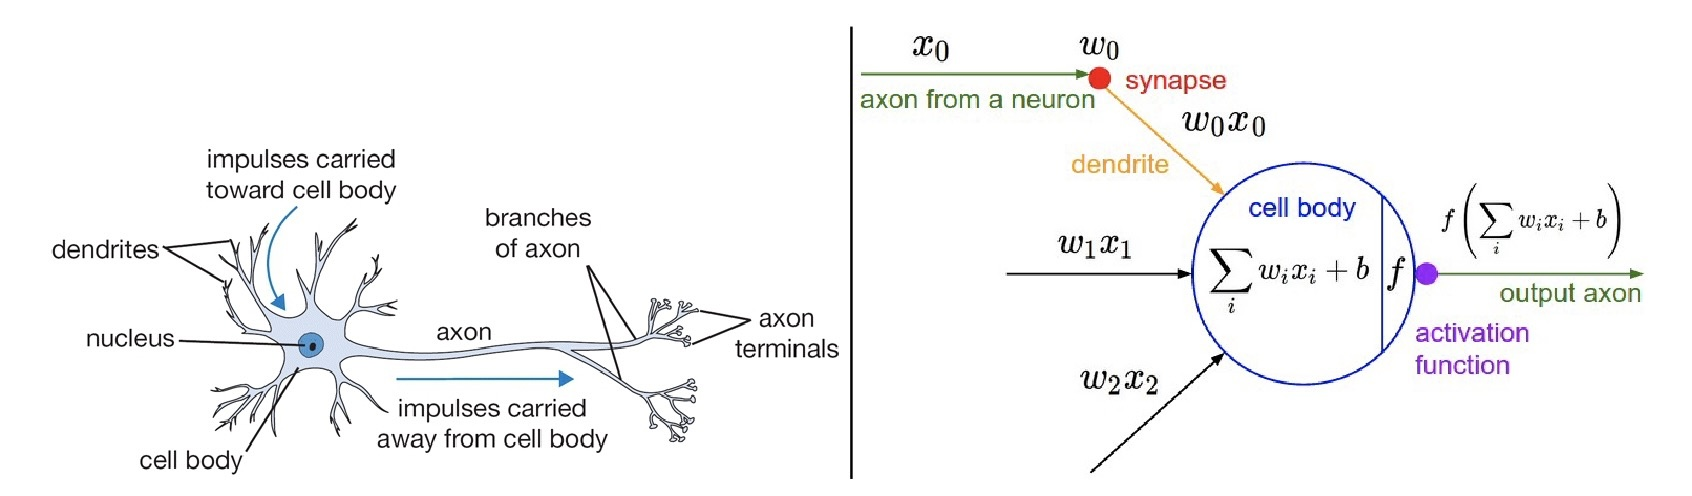
\includegraphics[width=1\linewidth]{figs/chapter3/neuron.jpg}
    \vspace{-3ex}
\end{figure}

\paragraph{常用激活函数} \hspace{1ex}

\begin{table}[H]
    \centering
    \small
    \begin{tabularx}{0.7\linewidth}{XX}
        \toprule
        名称 & 表达式 \\
        \midrule
        Sigmoid & $\sigma(x)=\frac{1}{1+e^{-x}}$ \\
        Tanh & $\tanh(x)=\frac{e^x-e^{-x}}{e^x+e^{-x}}$ \\
        ReLU & $f(x)=\max(0,x)$ \\
        Leaky ReLU / PReLU & $f(x)=[x<0](\alpha x)+[x\geqslant 0]x$ \\
        Maxout & $f(x)=\max(w_1x+b_1,w_2x+b_2)$ \\
        \bottomrule
    \end{tabularx}
\end{table}

\begin{itemize}
    \item Sigmoid：函数曾经很常用，但最近很少用了，这是因为它有两个大弊端：
    \begin{itemize}
        \item Sigmoids 会 saturate，导致\textbf{梯度消失}。由于 $\sigma(x)$ 在 $|x|$ 较大时梯度非常小，而神经网络反向传播的本质是链式求导法则，要把梯度一级一级地乘起来，所以一旦遇到梯度很小的地方，梯度就无法继续反向传播了，这将导致前层的神经元的参数几乎不怎么更新。
        \item Sigmoid 的输出不是以 $0$ 为中心的，这意味着后一层神经元接受的输入都是大于 $0$ 的数，从而导致参数 $w$ 的梯度全为正或者全为负。
    \end{itemize}
    \item Tanh: $\tanh(x)=2\sigma(2x)-1$，所以依然存在梯度消失的问题。
    \item ReLU：
    \begin{itemize}
        \item (+) 与 sigmoid 或 tanh 相比，ReLU 大大加速了 $\text{SGD}$ 的收敛速度；
        \item (+) ReLU 的计算非常简单，而 sigmoid 和 tanh 涉及到指数等比较耗时的计算；
        \item (-) 使用 ReLU 容易导致神经元“死亡”. 如果学习率设置的过大，容易使得参数变化过大，导致对数据集中的所有点 $wx+b$ 都小于 $0$，于是梯度不可逆地变成 $0$.
    \end{itemize}
    \item Leaky ReLU：为了解决 ReLU 中神经元“死亡”的问题，引入一个小常数 $\alpha$.
    \item PReLU：Leaky ReLU 中的 $\alpha$ 被视作神经元的一个参数参与优化。
    \item Maxout：ReLU / Leaky ReLU 是 Maxout 的特殊情况。
\end{itemize}


\paragraph{单神经元实现线性分类器}

选取合适的损失函数后，一个神经元可以用来实现一个 linear classifier.

\begin{itemize}
    \item \textbf{Binary Softmax classifier}：视神经元的输出 $\sigma\left(\sum_iw_ix_i+b\right)$ 为分类为正类的概率，采取 cross-entropy loss 训练，则得到 binary Softmax classifier，也即逻辑回归.
    \item \textbf{Binary SVM classifier}：使用 max-margin hinge loss 训练，则得到 Binary SVM.
\end{itemize}

\subsection{Neural Network Architectures}

一个输入层，一个输出层，若干隐藏层。对于最普通的神经网络而言，层与层之间全连接。
输出层的神经元经常没有激活函数，这样输出可以被视作分类的得分或者一些取实值的目标（比如回归值）。

\begin{figure}[H]
    \centering
    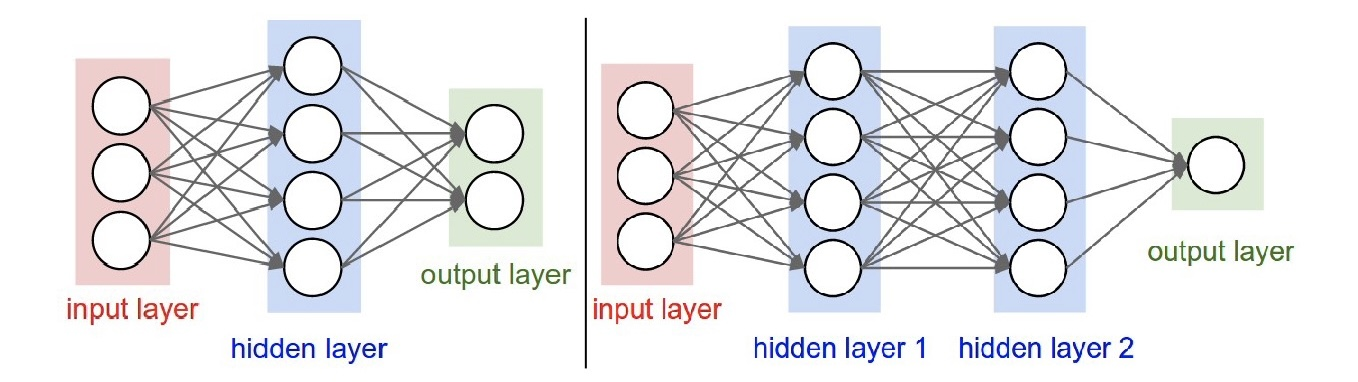
\includegraphics[width=0.8\linewidth]{figs/chapter3/neural network.jpg}
\end{figure}

单层神经网络可以以任意精度近似任何函数，严格证明在 Approximation by superpositions of a sigmoidal function (1989) 这篇论文中，直观解释可以在博客 \href{http://neuralnetworksanddeeplearning.com/chap4.html}{Neural Networks and Deep Learning} 中找到。虽然如此，实践中多层的神经网络效果更好，也更容易学习。

神经网络中，隐藏层神经元数量越多，其表达能力越强大：

\begin{figure}[H]
    \centering
    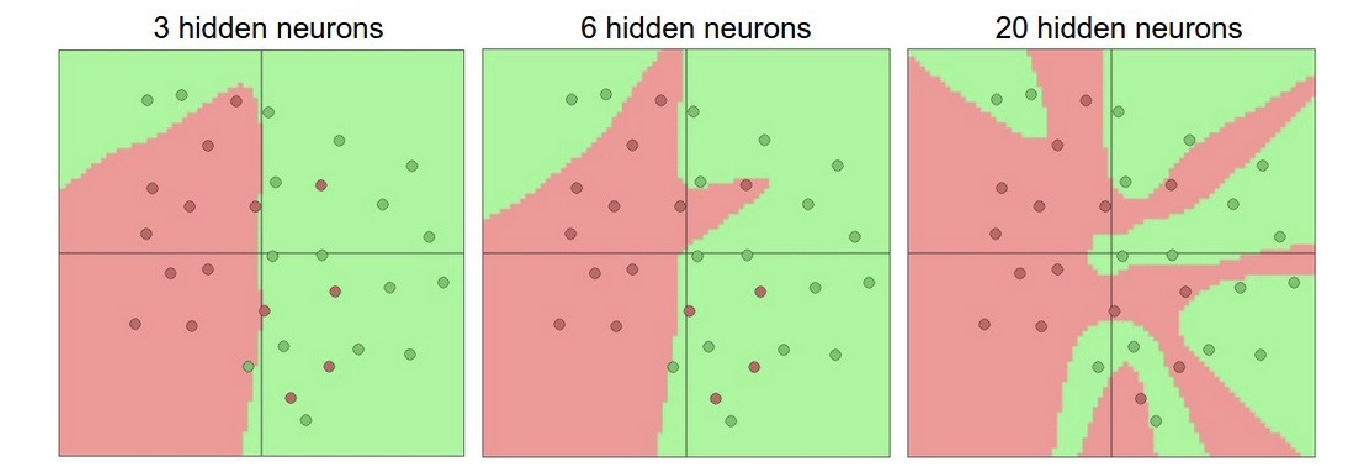
\includegraphics[width=0.7\linewidth]{figs/chapter3/hidden neurons.jpg}
\end{figure}

但这也意味着越容易过拟合，可以采取正则化的方式避免过拟合：

\begin{figure}[H]
    \centering
    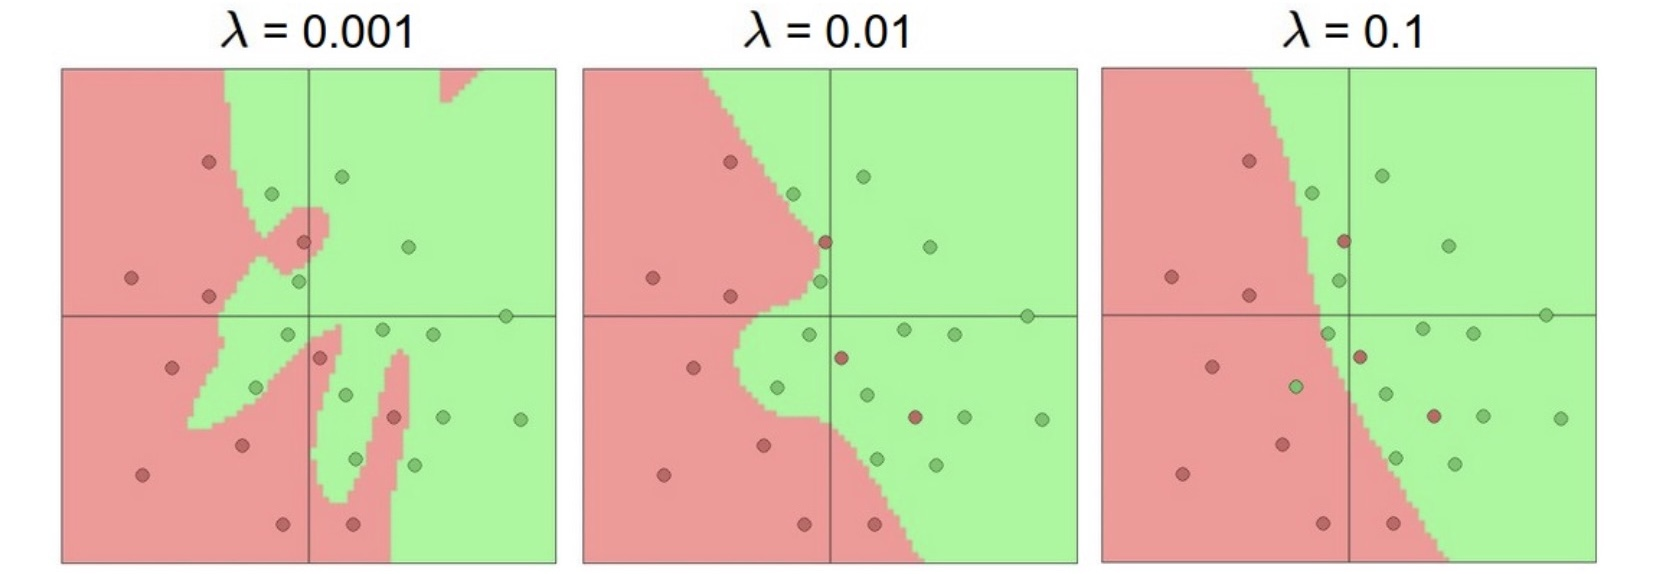
\includegraphics[width=0.7\linewidth]{figs/chapter3/overfitting.jpg}
\end{figure}

\subsection{Data Preprocessing}

\paragraph{Mean subtraction}
将所有数据减去平均值，即中心化。

\paragraph{Normalization}
将数据的各维度缩放到大致相同的规模。一般有两种方式：一是对中心化后的数据除以各维度的标准差，使得各维度的数据均值为 $0$，方差为 $1$；二是将最大值和最小值缩放为 $1$ 和 $-1$，这样所有数据都在 $[-1,1]$ 之中。
\begin{figure}[H]
    \centering
    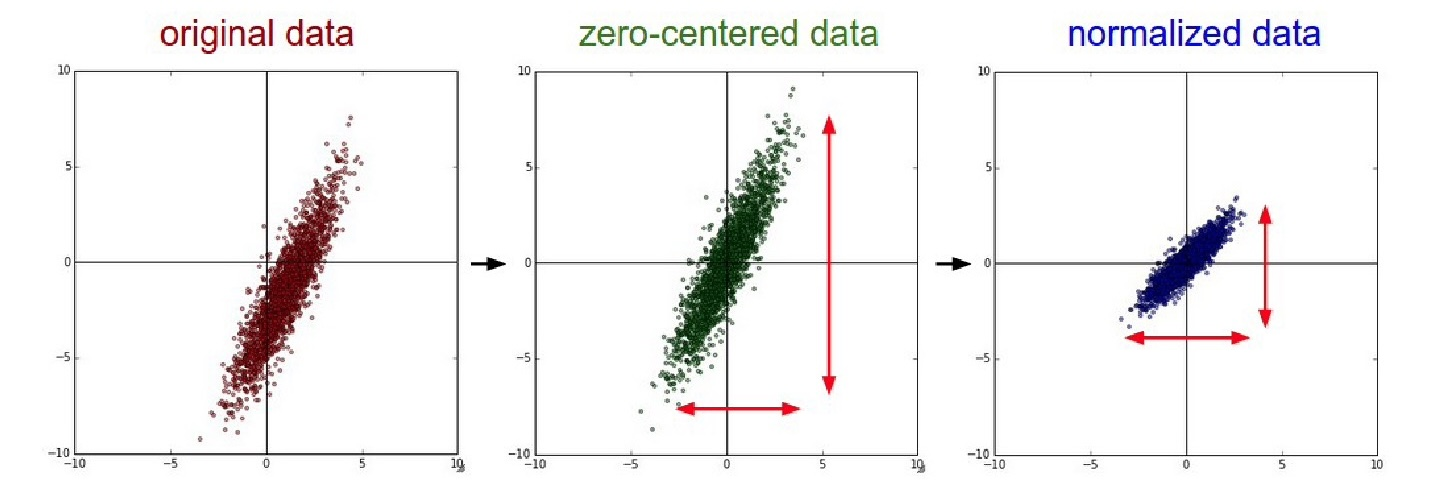
\includegraphics[width=0.8\linewidth]{figs/chapter3/data.jpg}
\end{figure}

\paragraph{PCA}
主成分分析 (PCA) 是一种常用的数据降维方法，具体内容可见机器学习笔记。

\paragraph{Whitening}
假设数据是一个多元高斯分布，则 whitening 将数据变为均值为 $0$，协方差矩阵为单位矩阵的多元高斯分布。就具体实现而言，在主成分分析中，如果没有使维度减小，则其效果为去相关性 (decorrelate)；对去相关性后的数据除以各维度的特征值就得到了 whitening 的数据。
\begin{figure}[H]
    \centering
    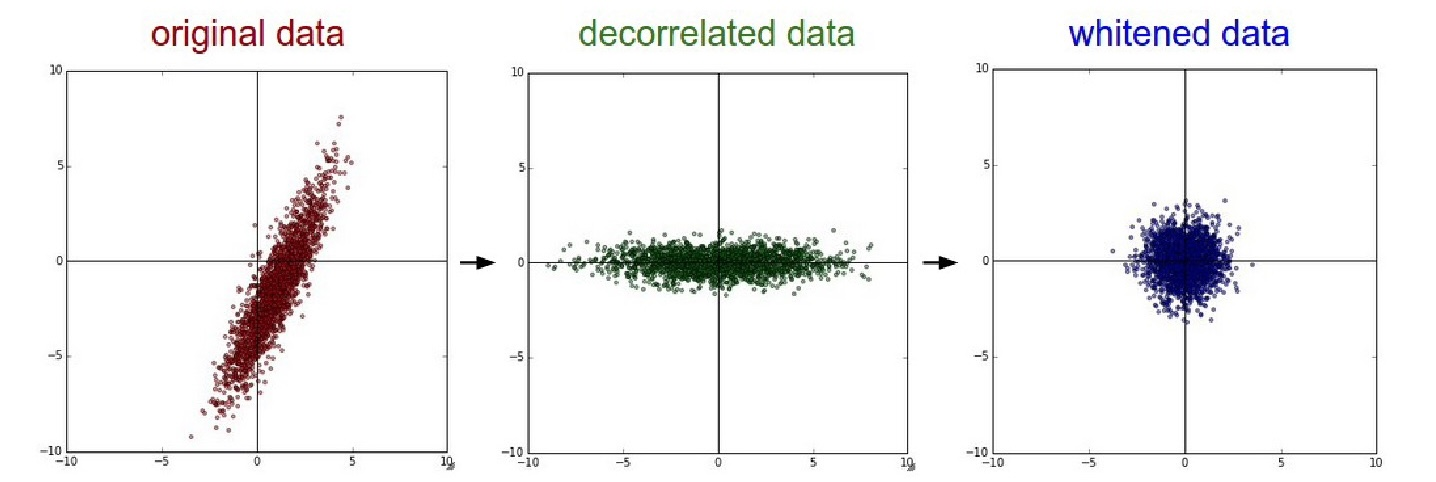
\includegraphics[width=0.8\linewidth]{figs/chapter3/whiten.jpg}
\end{figure}

\begin{com}
卷积神经网络一般不采用 PCA 和 whitening，但是中心化以及 normalization 很重要。
\end{com}

\begin{note}
在数据预处理时，预处理的统计量应该由训练集计算而来，然后应用到验证集或测试集上。\textbf{不能够}先在整个数据集上预处理，再划分训练/验证/测试集。
\end{note}

\subsection{Weight Initialization}

\paragraph{全零初始化（陷阱）}
全部初始化为 $0$ 是错误的做法，因为这样同一层的所有神经元都没有区别，它们将输出同样的值、具有同样的梯度、进行同样的更新（因为它们是对称的），这是没有意义的。

\paragraph{小随机数}
初始化为接近 $0$ 的随机数是经常使用的方法。一般而言，可以取 $0.01$ 倍的标准正态分布或者均匀分布等。

\paragraph{方差修正}
上一个方法存在一个问题，即神经网络输出的方差将随着输入量的增大而增大。在 \href{http://neuralnetworksanddeeplearning.com/}{Neural Networks and Deep Learning} 中作者举了一个\href{http://neuralnetworksanddeeplearning.com/chap3.html\#weight\_initialization}{例子}说明这一点：不妨假设 $1000$ 个输入中有 $500$ 个 $0$ 和 $500$ 个 $1$，考察第一个隐藏层中的一个神经元，$z=\sum_jw_jx_j+b$ 将是 $501$ 个标准正态分布之和，故服从 $N(0,501)$，方差高达 $501$. 为了解决这个问题，我们计算：
\begin{align*}
\var(z)&\approx\var\left(\sum_jw_jx_j\right)&&\text{for simplicity, ignore bias}\\
&=\sum_{j}\var(w_jx_j)&&\text{independence}\\
&=\sum_j(\E [w_j])^2\var(x_j)+(\E[x_j])^2\var(w_j)+\var(x_j)\var(w_j)\\
&=\sum_j\var(x_j)\var(w_j)&&\text{assume }\E(x)=\E(w)=0\\
&=n\ \var(w)\ \var(x)
\end{align*}
因此，若要 $\var(z)=\var(x)$，需要 $\var(w)=1/n$，故我们只需要将初始化的值除以 $1/\sqrt n$ 即可。实践中这样做能加快收敛。
\begin{com}
    在 \href{https://proceedings.mlr.press/v9/glorot10a/glorot10a.pdf}{Understanding the difficulty of training deep feedforward neural networks} by Glorot et al. 这篇论文中，作者最终建议用 $\var(w)=2/(n_\text{in}+n_\text{out})$ 来初始化；在 \href{https://arxiv.org/abs/1502.01852}{Delving Deep into Rectifiers: Surpassing Human-Level Performance on ImageNet Classification} by He et al. 中，作者对 ReLU 神经网络进行分析，得到结论是方差应初始化为 $2/n$.
    
    \textbf{实践中，建议采用 ReLU 神经元并将权重方差设为 $2/n$.}
\end{com}

\paragraph{稀疏初始化}
另一种初始化方式是将权重矩阵初始化为 $0$，但是为了打破对称性，每个神经元随机地连接下一层若干神经元（连接数目可由一个小的高斯分布生成）。

\paragraph{偏置初始化}
偏置项常初始化为 $0$.

\paragraph{Batch Normalization}
在全连接层/卷积层与 激活函数 之间插入一个 BatchNorm layer，因为 normalization 是可导的操作，这么做是可行的，具体查看论文：\href{https://arxiv.org/abs/1502.03167}{Batch Normalization: Accelerating Deep Network Training by Reducing Internal Covariate Shift}.


\subsection{Regularization}

\paragraph{L2 正则化}
最常见的正则化方法，向损失函数加上 $\frac{1}{2}\lambda w^2$. 其特点是使得网络倾向于分散的权重。

\paragraph{L1 正则化}
相对常见的正则化方法，向损失函数加上 $\lambda |w|$. 其特点是使得网络的权重倾向于稀疏（即许多非常接近 $0$ 的数字，与 L2 正好相反）。结合 L1 和 L2 可得 Elastic net regularization，即向损失函数加上 $\lambda_1|w|+\lambda_2 w^2$. 一般而言，如果不是特别关注某些特征的选择，L2 比 L1 效果会更好。

\paragraph{最大范数约束}
给神经元的权重向量 $w$ 以约束：$||w||_2<c$，$c$ 一般取 $3$ 或 $4$。

\paragraph{Dropout}
及其有效和简单的正则化方法，在 \href{https://www.cs.toronto.edu/\%7Ersalakhu/papers/srivastava14a.pdf}{Dropout: A Simple Way to Prevent Neural Networks from Overfitting} by Srivastava et al. 中提出，能作为其他正则化方法的补充。实现方法是在训练中让神经元以概率 $p$（一个超参数）激活或设置为 $0$.

\begin{figure}[H]
    \centering
    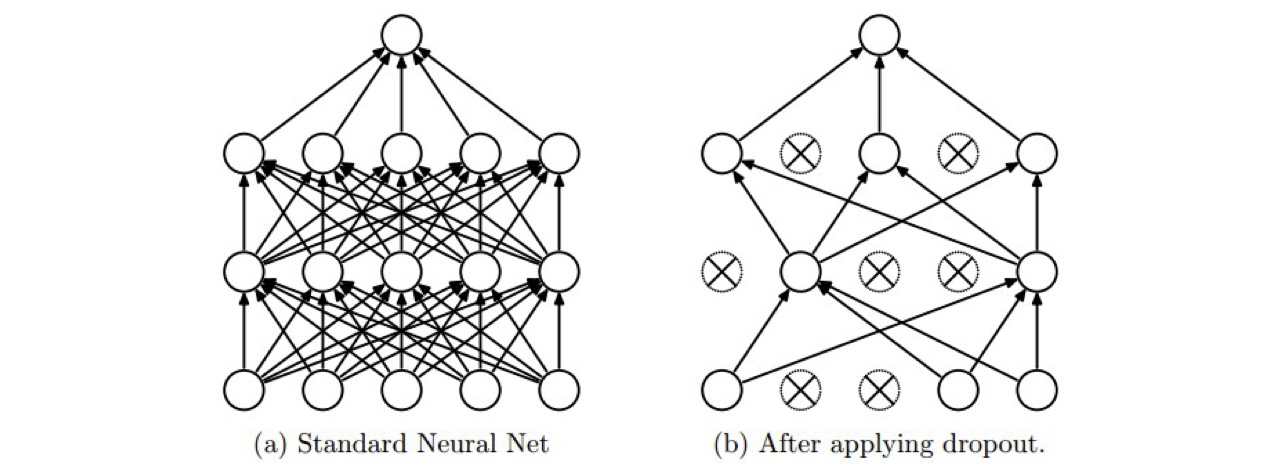
\includegraphics[width=0.8\linewidth]{figs/chapter3/dropout.jpg}
\end{figure}

\paragraph{偏置项}
偏置项没有与数据直接相乘，因此无需正则化，即便正则化对结果的影响也微乎其微。

\subsection{Loss Functions}

\paragraph{分类}

常用 SVM loss:
\[
L_i=\sum_{j\neq y_i}\max(0,f_j-f_{y_i}+1)
\]
和 cross-entropy loss:
\[
L_i=-\ln\left(\cfrac{e^{f_{y_i}}}{\sum_je^{f_j}}\right)
\]

\paragraph{属性分类}

不一定被分为某一类，而可以分到若干类，设 $y_{ij}$ 表示第 $i$ 个图像是否属于第 $j$ 类。我们可以对每一类训练一个 logistic regression classifier，然后用负的对数似然作为损失函数：
\[
L_i=-\sum_j y_{ij}\ln\sigma(f_j)+(1-y_{ij})\ln(1-\sigma(f_j))
\]

\paragraph{回归}

可采取 L2 或 L1 距离作为损失函数，即：
\[
L_i=||f-y_i||_2^2=\sum_j(f_j-(y_{i})_j)^2
\]
或
\[
L_i=||f-y_i||_1=\sum_j|f_j-(y_i)_j|
\]

\subsection{Gradient Checks}

神经网络反向传播过程很容易写出 bug，为了检验我们计算的梯度是否正确，可以将解析梯度和数值梯度进行比较。这里有一些实现的 tips：

\begin{itemize}
    \item 计算 numerical gradient 时，使用 centered formula，即：
    \[
    \frac{\mathrm df(x)}{\mathrm dx}\approx\frac{f(x+h)-f(x-h)}{2h}
    \]
    而非 $\frac{\mathrm df(x)}{\mathrm dx}\approx\frac{f(x+h)-f(x)}{h}$，这是因为前者误差为 $O(h^2)$，而后者有 $O(h)$. （泰勒展开即可证）

    \item 使用相对误差作为比较基准。如果使用绝对误差，比如 $10^{-4}$，那么在梯度本来就小于 $10^{-4}$ 的地方，这个阈值没有什么作用。因此，我们使用相对误差：
    \[
    \frac{|f'_{\text{analytic}}-f'_\text{numerical}|}{\max\left(|f'_\text{analytic}|,|f'_\text{numerical}|\right)}
    \]
    分母用 $\max$ 或者加和或者取任意一个都是可以的，但是要小心除零。

    \item 注意目标函数的不可导点。跨越了不可导点的 numerical gradient 可能和实际的 gradient 有较大差距，如果误差较大需要检查是不是这个原因。

    \item 只使用少量数据。解决上一条问题的一个方法是 gradient checks 时只用少量的数据，这样目标函数的不可导处将减少；同时只用检验 $2\sim3$ 处的梯度就够了。

    \item $h$ 不宜设置得太小。理论上 $h$ 越小越精确，但由于计算机浮点数的精度误差，太小了可能反而不精确。

    \item 小心正则化项占了梯度的主要部分。如果正则化项在梯度中占比很大，它可能掩盖住了 back propagation 的错误。一个方式是在梯度检验时去掉正则化。

    \item 记住去掉 dropout/augmentations. 梯度检验时需要去除带有\textbf{随机性质}的量，比如 dropout 或者数据的随机 augmentation. 提前设置一个随机数种子也是可以的。

\end{itemize}

\subsection{Sanity Checks}

在开始训练之前，可以先进行 sanity checks，以保证我们的代码是正确的。

\begin{itemize}
    \item 按概率推测损失函数初始值。例如一个十分类问题，随机初始化后我们应期望得到 $1/10$ 的正确率，也即负对数概率的损失函数大致为：$-\ln(0.1)=2.302$.
    \item 过拟合一个极小的数据集。用一个极小的数据集去训练，在去除正则化的情况下，我们应该期望得到 $100\%$ 的正确率或损失函数为 $0$，即在这个极小的数据集上过拟合。

\end{itemize}

\subsection{Babysitting the learning process}

学习过程中我们可以监测一些值随着迭代次数的增加的变化。

\begin{itemize}
    \item \textbf{Loss function}. 作 loss - epoch 图能直观的告诉我们学习的状况，帮助我们调整学习率等参数。

    \begin{figure}[H]
        \centering
        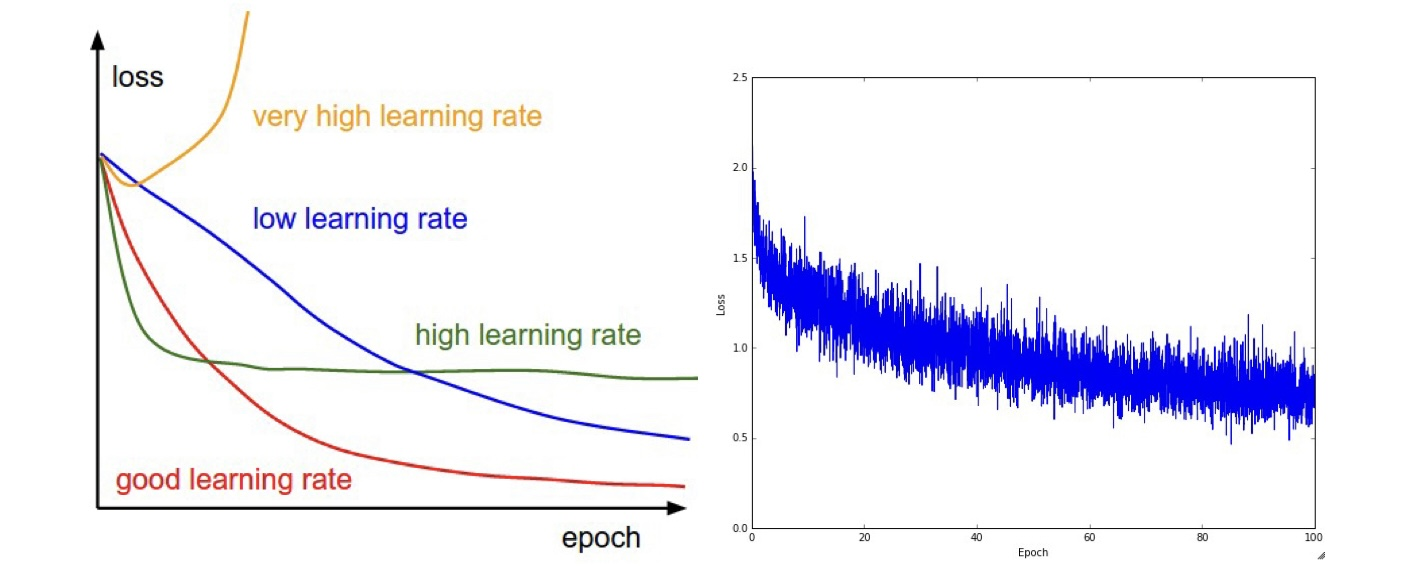
\includegraphics[width=0.8\linewidth]{figs/chapter3/loss.jpg}
    \end{figure}

    \item \textbf{Train/val accuracy}. 作训练集和验证集上的准确率的图能直观的告诉我们是否过拟合/欠拟合，帮助我们调整正则化项。

    \begin{figure}[H]
        \centering
        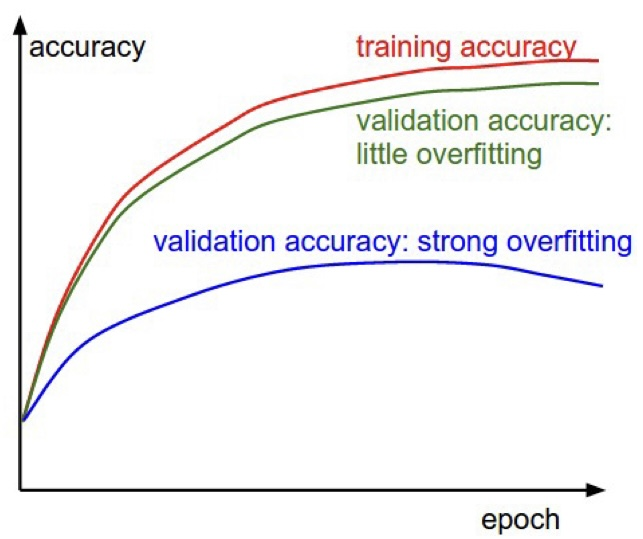
\includegraphics[width=0.4\linewidth]{figs/chapter3/train val accuracy.jpg}
    \end{figure}

    \item \textbf{Ratio of weights updates}. 检测参数更新的幅度，帮助我们判断学习率是否合适，合适的幅度应该在 $10^{-3}$ 左右。

    \item \textbf{First-layer Visualizations}. 在图像处理的网络中，我们可以把第一层的神经元的参数还原成图像可视化。

    \begin{figure}[H]
        \centering
        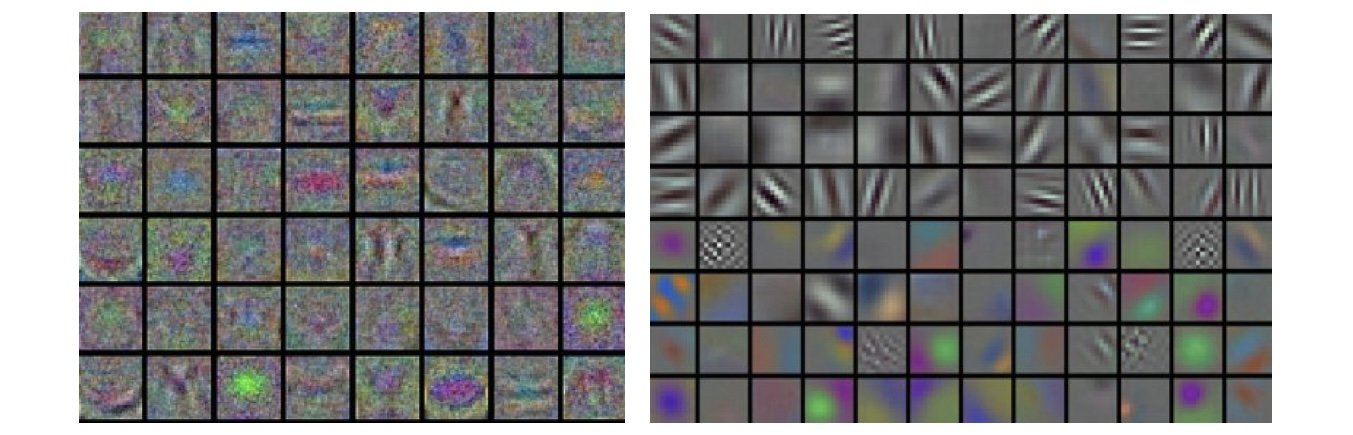
\includegraphics[width=0.8\linewidth]{figs/chapter3/first.jpg}
    \end{figure}

\end{itemize}


\subsection{Parameter updates}

\paragraph{SGD 及其延伸}

\begin{itemize}
    \item \textbf{Vanilla update}. 朴素的随机梯度下降

    \item \textbf{Momentum update}. 朴素的 SGD 在每一处都向梯度下降的方向更新，就像一个人下山一样。而如果我们做另一个比喻，想象一个小球从山坡滚下，它在每一处将具有保持原方向的惯性，这就是 momentum SGD 的灵感来源。具体地，momentum SGD 更新如下：
    \begin{align*}
    v&:=\mu v-\alpha\ \mathrm dx\\
    x&:=x+v
    \end{align*}
    其中，$\alpha$ 为学习率，$\mu$ 可以看作是摩擦因子。

    \item \textbf{Nesterov Momentum}. 这是另一种 momentum update. 不同于上一条，Nesterov Momentum 计算随“惯性”移动一段距离之后的梯度再更新，见下图：

    \begin{figure}[H]
        \centering
        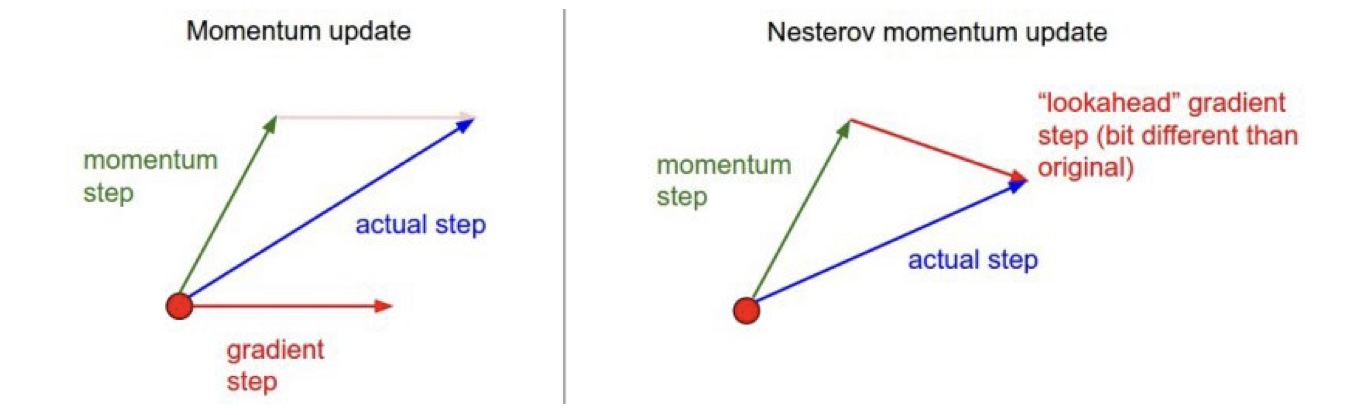
\includegraphics[width=0.8\linewidth]{figs/chapter3/momentum.jpg}
    \end{figure}

    具体地，Nesterov Momentum 更新如下：
    \begin{align*}
    x_\text{ahead}&:=x+\mu v\\
    v &:= \mu v-\alpha\ \mathrm dx_\text{ahead}\\
    x&:=x+v
    \end{align*}
\end{itemize}

\paragraph{学习率退火}

在学习过程中不断减小学习率往往有帮助，一下三种方式是常用的 learning rate decay 实现方式：

\begin{itemize}
    \item \textbf{Step decay}. 每迭代几次后将 learning rate 减小，例如每 $20$ 次迭代后减小到原来的 $0.1$，或者每 $5$ 次迭代减小一半等。这些参数依赖于具体问题和模型。一种启发式方法是当 validation error 停止减小时就减小 learning rate.
    \item \textbf{Exponential decay}. 依 $\alpha=\alpha_0e^{-kt}$ 减小，其中 $\alpha_0,k$ 是超参数，$t$ 是迭代次数。
    \item $1/t$ \textbf{decay}. 依 $\alpha=\alpha_0/(1+kt)$ 减小。
\end{itemize}
实践中，step decay 稍稍更受喜爱一些，因为其解释性比其他的强。

\paragraph{二阶方法}

梯度下降及其延伸算法只需要用到一阶导数，即梯度。还有些最优化算法需要用到二阶导数。
例如 Newton's method：
\[
x:=x-[Hf(x)]^{-1}\nabla f(x)
\]
其中，$Hf(x)$ 表示 Hessian matrix，$\nabla f(x)$ 表示 $f(x)$ 的梯度向量。

注意到上述更新中不含有学习率这一超参数，这也是其优于一阶方法所在。
但是，Newton's method 有一个及其显著的缺点，即 Hessian matrix 过于庞大，$n$ 个参数的 Hessian matrix 是 $n\times n$ 的，计算耗时且难以存储。因此，出现了众多 quasi-Newton methods，例如 $\text{L-BFGS}$，它们不需要将 Hessian matrix 完整计算出来.

\paragraph{逐参数自适应学习率}

在之前的算法中，学习率是全局的且对所有参数都一样。调整学习率是一个耗时耗力的过程，因此人们发明了许多自动调整学习率的方法，且这些学习率甚至能对每一个参数进行调整。
虽然这些方法也有超参数，但它们与纯粹的学习率相比，能在更大的范围内表现较好，因而更好调参。

\begin{itemize}
    \item \textbf{Adagrad}：
    \begin{align*}
    \text{cache}&:=\text{cache}+(\mathrm dx)^2\\
    x&:=x-\alpha\ \frac{\mathrm dx}{\sqrt{\text{cache}}+\text{eps}}
    \end{align*}
    注意，上式中对向量的运算符定义为与 \texttt{numpy} 相同。
    对上式的理解是：$\text{cache}$ 一路记录了每个参数的梯度平方和，如果某个参数有较大的梯度，那么它的学习率将减小；相反，梯度较小的参数将有较大的学习率。

    \item \textbf{RMSprop}：RMSprop 在 Adagrad 的基础上进行了简单的修改：
    \begin{align*}
    \text{cache}&:=\text{decay rate}\times \text{cache}+(1-\text{decay rate})\times (\mathrm dx)^2\\
    x&:=x-\alpha\ \frac{\mathrm dx}{\sqrt{\text{cache}}+\text{eps}}
    \end{align*}
    也即是增加了 $\text{decay rate}$ 这一超参数，一般取值为 $0.9,0.99,0.999$.

    \item \textbf{Adam}：可以看作是 RMSprop 带 momentum 的版本，其（简化的）更新如下：
    \begin{align*}
    m&:=\beta_1m+(1-\beta_1)\mathrm dx\\
    v&:=\beta_2v+(1-\beta_2)(\mathrm dx)^2\\
    x&:=x-\alpha\ \frac{m}{\sqrt{v}+\text{eps}}
    \end{align*}
    典型的参数是：$\text{eps}=10^{-8},\beta_1=0.9,\beta_2=0.999$.

    完整的 Adam 算法存在一个 bias correction 机制：
    \begin{align*}
    m&:=\beta_1m+(1-\beta_1)\mathrm dx\\
    \color{purple}{mt}&\color{purple}{:={m}/({1-\beta_1^t})}\\
    v&:=\beta_2v+(1-\beta_2)(\mathrm dx)^2\\
    \color{purple}{vt}&\color{purple}{:=v/(1-\beta_2^t)}\\
    x&:=x-\alpha\ \frac{\color{purple}{mt}}{\sqrt{\color{purple}{vt}}+\text{eps}}
    \end{align*}

\end{itemize}

\subsection{Hyperparameter optimization}

超参数的优化是一个黑盒优化问题，其优化的目标函数是神经网络的性能，因而有一个显著的特点：得到每一组超参数的结果会花费巨额的时间。因此我们并不能直接套用一般的优化方法对超参数进行优化。一般的，超参数优化方法有以下几种：

\begin{itemize}
    \item \textbf{网格搜索}：即每个超参数设置几个值，暴力遍历所有的可能。

    \item \textbf{随机搜索}：在论文 \href{https://www.jmlr.org/papers/volume13/bergstra12a/bergstra12a.pdf}{Random Search for Hyper-Parameter Optimization} by Bergstra and Bengio 中，作者论证了随机搜索比暴力遍历更为优秀，且更容易实现。

    \begin{figure}[H]
        \centering
        
\includegraphics[width=0.8\linewidth]{figs/chapter3/grid.jpg}
    \end{figure}

    \item \textbf{贝叶斯超参数优化}：利用贝叶斯方法进行超参数的寻找。

\end{itemize}

\subsection{Model Ensembles}

实践中，一个提升神经网络性能的方法是训练多个独立的模型，使用它们的平均预测结果。这些独立的模型可以是不同的模型，同一种模型、不同初始化条件，甚至是同一个模型在训练的不同时间点处等。除了对模型结果进行平均，还可以对各模型的参数进行平均，有时也能提高神经网络性能。
